
\chapter{INTRODUCTION}


\section{Harmful Algal Blooms}


 %First paragraph. INTRODUCTION GENERIC PARAGRAPH


\gls{hab} are disastrous events which has impacted multiple areas around the world. With \gls{hab}, algae and cyanobacteria can grow out of control, often ``painting'' the water green. \gls{hab} are a result of over-productivity of phytoplankton biomass which mostly resides in the epipelagic zone often forming a thick layer \cite{moore_richard_cyanobacterial_1993}.  In most cases, \gls{hab} are found in coastal regions, streams, and freshwater lakes \cite{rastogi_cyanotoxin-microcystins:_2014}. The composition of
\gls{hab} are diverse ranging from  different species of cyanobacteria, diatoms, algae, and dinoflagellates found worldwide \cite{dittmann_cyanobacterial_2012}.  Unfortunately, the intensity, extent, and spatial coverage of \gls{hab} has been increasing globally due to more ecological disturbances \cite{codd_cyanobacterial_1999}. A prime example would be the case of Lake Erie as it has face decades of abuse. Historically, Lake Erie  In 2014, Lake Erie was faced with \gls{hab}, in particular with \emph{Microcystis aeruginosa}, affected over 400,000 people, hindering drinking water supply in Toledo, Ohio which prevented residents to drink or bath in their homes \cite{mann_toledo_2014}.
The Laurentian Great Lakes are a vital source of freshwater. The Great Lakes holds 20\% of the worlds freshwater which is most arguably the most important resource for human life \cite{carmichael_health_2016}. It would be tragic to fail in protecting the Great Lakes.



Swimming or contact in any waterbody with \gls{hab} can pose a health risk as some \gls{hab} can have toxin producing species. Many of the species that are producing hepatoxins and neurotoxins in high amounts are killing livestock and wildlife \cite{anderson_harmful_2002}. The possible route of exposure  for humans can be from dermal contact, accidental ingestion, breathing in lake spray aerosols and failure of decontamination in drinking water plants \cite{may_aerosol_2018,codd_cyanobacterial_1999}. Exposure through dermal contact can be an irritant. \gls{hab} can create lipopolysaccharide, an endotoxic, which create rashes on upon contact with skin as it triggers a inflammatory response \cite{ moore_richard_cyanobacterial_1993}. Although a rare case, accidental ingestion of cyanotoxin by directly drinking water from an affected lake could  lead to acute toxicity or other symptoms \cite{monks_potent_2007}. However, there are \gls{hab} found in storage reservoirs in regions that do not have the sophisticated facility in providing clean water.

The harm caused by \gls{hab} does not necessarily come entirely from the toxins. In cases of \gls{hab} where large accumulation biomass has peaked, they can quickly die off due to limiting resources \cite{charlton_oxygen_1980}. The dead biomass is quickly consumed by other aquatic microorganisms which increases respiration rates, depletes dissolved oxygen creating an unsuitable habitat for higher-ordered aquatic mammals.  \cite{anderson_harmful_2002}.
The layer of scum formed from \gls{hab} also block light for submerged aquatic macrophytes, killing them by dissallowing photosythesis \cite{ bucak_modeling_2018}. \gls{hab} can also be a major nuisance and a cost to commodity, as it creates odor and detract recreational swimmers  \cite{graham_cyanotoxin_2010, carmichael_health_2016}.




%Toxicity
Cyanobacterial toxins (cyanotoxins) are vastly diverse as 600 recognized peptides have been discovered \cite{welker_cyanobacterial_2006}. The variety of toxins have a range of different mechanism of toxicity. One of the most dangerous called saxitoxin are sodium channel blockers, a potent neurotoxin which paralyze and dead from respiratory failure \cite{moore_richard_cyanobacterial_1993}.
Anatoxin-a is also a very dangerous with its potent toxicity. It is known as Very Fast Death Factor due to its ability to irreversibly bind to nicotinic acetylcholine receptors which consequently leading to respiratory failure in a very quickly manner \cite{codd_cyanobacterial_1999, moore_richard_cyanobacterial_1993}. Cyanotoxins are mostly intracellular, except for the case of cylindrospermonspin \cite{rastogi_cyanotoxin-microcystins:_2014}.



%Microcystin Toxicity
\gls{mc}, much of what our survey is focused on, is a small cyclic peptide having a large range of diverse structure. The mode of toxicity is its ability to inhibit protien phosphatases 1, 2A and 3 \cite{moore_richard_cyanobacterial_1993} MC is produced mostly by \emph{Microcystis aeruginosa} but also by few other species such as \emph{Anabaenopsis, Cylindrospermopsis, Nostoc,} and \emph{Planktrothrix} \cite{rastogi_cyanotoxin-microcystins:_2014, davis_phylogenies_2014}.

%Microcystin synthesis
Microcystins are uniquely produced by a mix of two systems, \gls{pks} and  \gls{nrps} \cite{tillett_structural_2000}. This is different from how other protiens are normally synthesized ribosomally . The genetic mechanism of MC synthesis involves multiple protein modules spanning from 48 kilobase pair gene cluster which are responsible for incorporating different amino acids, ultimately creating the cyclic peptide \cite{moffitt_characterization_2004,nishizawa_genetic_1999}. The major amino residues of MC  are of \gls{dmeasp}, \gls{adda},  \gls{mdha} and other possible variable amino acids \cite{trogen_conformational_1996,nishizawa_genetic_1999}.
% Microcystin congener
There are over 100 known variation of MC with 6 congeners recognized by the \gls{epa} as chemical contaminants which are \gls{mcla}, \gls{mclf}, \gls{mclr}, \gls{mcly}, \gls{mcrr}, and \gls{mcyr} \cite{puddick_modulation_2016}. The most frequently occurring and potent congener variant of MC is MC-LR \cite{rastogi_cyanotoxin-microcystins:_2014}. Figure \ref{fig:structure1} shows the structure of MC-LR which contains L-luecine (L) and L-Arginine (R) in its variable positions. Other amino acids such as alanine (A), tryptophan (W), tyrosine (Y), and phenylalanine (F) can be substituted for other variable congeners.
With the known variants, MC is roughly around 1000 Da \cite{dittmann_cyanobacterial_2012}



 \begin{figure}[t]
   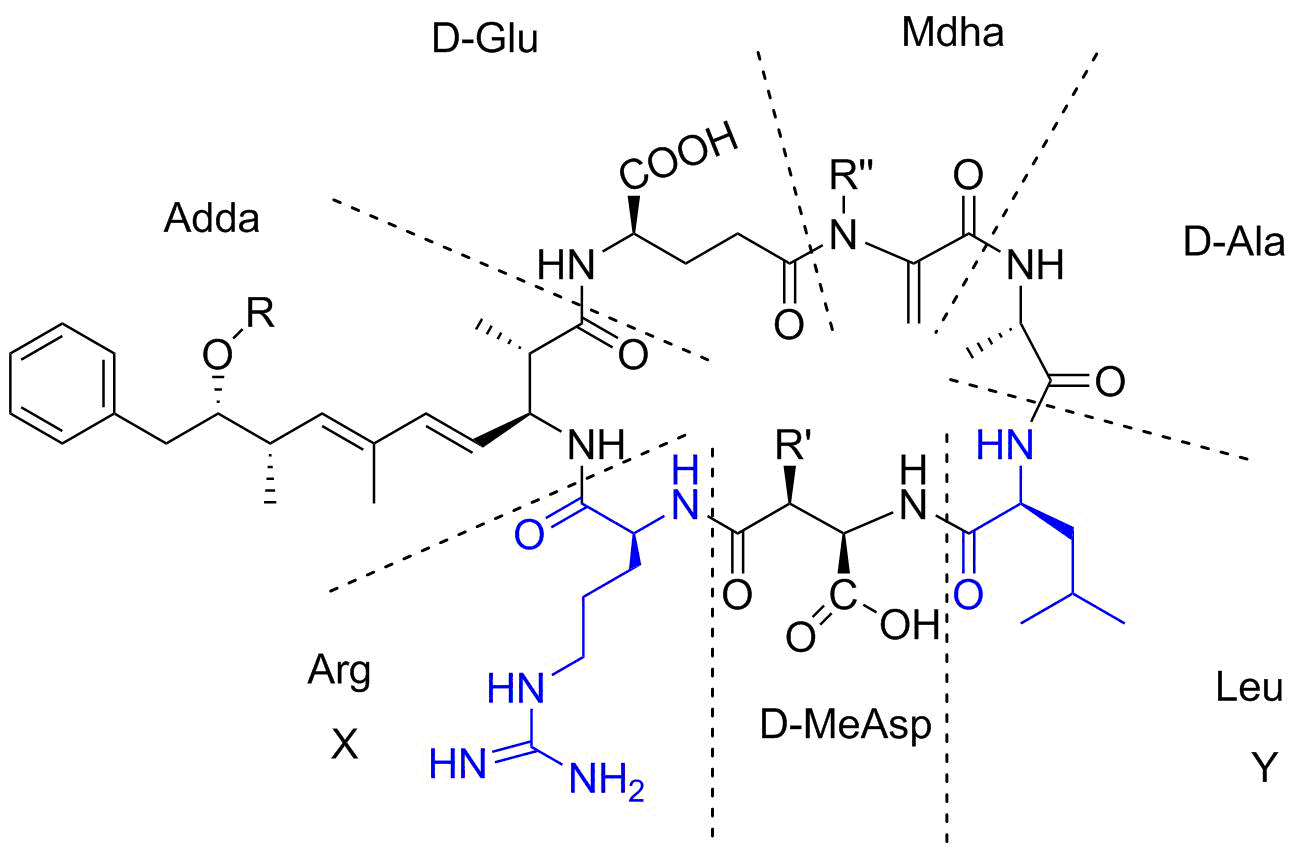
\includegraphics[width=\textwidth]{Microcystin-LR.eps}
   \caption{Structure of MC-LR}
   \label{fig:structure1}
   \begin{flushleft}
   a) Adda group
   b) L-leucine, a variable amino group amongst other congeners
   c) L-arginine, also a variable amino group in other congeners
   d) Methyl-group which can be demethylated in other congeners.
     \end{flushleft}

 \end{figure}

 %REGULATION
State officials continuously monitor and analyze surface and drinking water for cyanotoxins. The \gls{who} have a guidance level of 1 $\mu$g/L for drinking water \cite{world_health_organization_guidelines_2003} For the state of Michigan, the USEPA have a draft guidance level for recreational surface water of 4 $\mu$g/L \cite{usepa_draft_2016}. Methods of quantifying MC will often measure \gls{mclr}. Levels above those guidelines requires state officials to issue a health advisory not to swim in the effected area.  The common routine methods employed by state agencies are ELISA kits by Abraxxis. This is an antibody method that detect and measures the ADDA-moiety of the MC.
The test kit has good cross-reactivity with other congeners, and it uses \gls{mclr} for its calibration standards so the reported value is in terms of MC-LR equivalence.
%Ecological damage


%%%%%%%%%%%%%%%%%%%%%%%%%%%%%%%%%%%%%%%%%%%%
The mechanism for what drives the proliferation is not fully understood \cite{dittmann_cyanobacterial_2012}. As autotrophs, \gls{hab} can rapidly grow under warm and nutrient-rich conditions \cite{rastogi_cyanotoxin-microcystins:_2014}. \gls{hab} are most likely to occur in the summer or warmer months where primary productivity is most likely to peak due to increase daylight, warmer temperature and water flow in streams and rivers \cite{vannote_river_1980,chapra_climate_2017-2}



Eutrophication is one of the most prevalent issue in terms of causing \gls{hab}. Urbanization and agriculture has increased the frequency of  conditions in lakes and coastal environments, often regarded as cultural eutrophication\cite{smith_eutrophication_2009}.
Nutrients in the form of organic and inorganic forms play a role in biomass production. Nitrogen are usually from non-point sources from  septic tanks, animal waste and agricultural runoff which contributes to \gls{hab}. Nutrients from agriculture runnoff can have a great effect as fertilizer application has been increasing \cite{anderson_harmful_2002}. For the bloom in Lake Erie,
some studies suggests the culprit was due to the nutrient runnoff from the  Maumee river, which has and its watershed mostly comprised of agriculture \cite{michalak_record-setting_2013, chaffin_accuracy_2018}. Other studies in other areas worldwide, similar to Lake Erie, have shown nutrient enrich conditions usually from agricultural runoff or disturbance of ecological conditions that impacts nutrient cycle to cause blooms \cite{ahn_evaluation_2011, ahn_rainfall_2002, anderson_harmful_2002, jiang_statistical_2008}.

%FORMS OF NUTRIENTS%
In controlled lab experiments, nutrients such as inorganic nitrogen or phosphorus are found to be limiting growth factors. In a  when \emph{Microcystis aereginosa} grown in the laboratory \cite{xiao_colony_2018, yema_role_2016}.

Cyanobacteria are versatile as they can acquire nutrients under extreme conditions. They can utilize a process called quorom sensing which they coordinate with each other by using a signaling hormone acylated homoserine lactones \cite{van_mooy_quorum_2012}.
They also can create a network of cells which work together as a unit, often as seen as a layer of green goo floating on top of water.  There are very robust organisms, as some can change their buoyancy by modulating the intracellular gas vesicles gives them a competitive advantage over other species for seeking light \cite{feng_how_2018}.\emph{Microcystis} can form a complex colony made by a mucilage structure which can be bouyant due to high concentration of dissolved oxygen \cite{xiao_colony_2018}.


Most of the cyanotoxin are intracellular, however with increase turbulence from wind and precipitation can release more toxins due to cell lysis either from cell apoptosis or from mechanical abruption which release \cite{rohrlack_fate_2007}.



Ecological factors could be a major factor in some cases. Previous studies in inland Michigan lakes are finding New Zealand Mudsnails to have an impact on finding blooms \cite{vanderploeg_zebra_2001}.
In a study done by Michigan State University \cite{raikow_dominance_2004} found zebra mussels (\emph{Dreissena polymorpha}) can promote phytoplankton growth due to their effect on nutrient cycling. Some studies stress on the factor of zebra mussles if building a predictive model as it has a significant impact on \gls{hab} with their presence \cite{lavrentyev_effects_1995, knoll_invasive_2008, raikow_dominance_2004}. In our survey, we will investigate whether zebra mussels have an influence on MC concentration or cyanobacteria population.



%PREDICTIVE models
Predictive models are resourceful utility to forecast \gls{hab}. Models coupled with predicted weather  has increasingly been successful, with wind direction, speed, temperature and precipitation  has been effective in forecasting \gls{hab}. Along coastal environment,   \gls{noaa} uses real-time data from satellite to predict \gls{hab} on the Gulf of Mexico, Lake Erie, and other coastal environments based on satellite data and weather models \cite{kavanaugh_assessment_2013}.
Issuing warnings to the public can prevent exposure and be greatly beneficial. They have provide effective forecast, continuously available for the public on their website \footnote{\url{https://tidesandcurrents.noaa.gov/hab_info.html}}.

However, with inland lakes, satellite imagery is not ideal cloudy conditions. Forecasting for inland lakes does not work with satellite imagery as the extent of the lake's area will often limit the predictability.
An effective predictive models should be based on features that are found to contributes to \gls{hab} with measured abiotic and biotic factors.
Understanding the energy source for cyanobacteria can help to predict HAB occurrences.

---REALTIME DATA MODEL



 \section{Goals and Aims}

In our survey on 29 inland lakes in Michigan, we seek to build a predictive model on microcystins. In addition, we  measured for cylindrospermopsin and anatoxin-a to see if they are present in Michigan. Before the survey, I hypothesized if the lake's watershed is more urbanized areas I would expect higher MC concentrations. Developed land can increase nutrient rich runoff which can positive influence algal blooms. Previous studies shown developed areas having a major influence on the occurrence of \gls{hab} because of more possible sources like applied fertilizer or leaky septic tanks \cite{beaver_land_2014, anderson_harmful_2002}. Lakes with higher developed areas may also have a possible influence nutrient mobility, which in turn drive MC production.

One of our objectives is to have a model that is simple and robust in predicting \gls{hab}.
My goal is to explore what drives HAB development and build a predictive model based from our collected data.  With the collected observations, I investigated the best possible predictive model from our dataset.
Some studies build predictive models based using cyanobacterial cell count or mass, concentrations of chloraphyll-a and MC concentrations as a response variable as its most likely associated with \gls{hab} \cite{moore_richard_cyanobacterial_1993, ahn_evaluation_2011, jiang_statistical_2008, beaulieu_nutrients_2013, taranu_predicting_2017}.
%Cyanobacteria cell counts would be ideal to measure whether the lake is exhibiting a bloom.
The total MC concentration measured by \gls{lcmsms} was used as the main predictor variable of interest. The \emph{16s rRNA} gene copies measured by \gls{qpcr} was also observed as a response variables as well as this measures relatively amount cyanobacteria.



My research hypothesis:

\begin{enumerate}
 \item Harmful algal blooms are influenced by  developed/urban land, which can be used to predict MC concentrations
 \item Lakes with the presence of zebra mussel will have a higher concentration of MC than lakes with none found.
 \item Nutrient concentrations can be explained by land use characteristics
 \item Identify important features from the collected dataset to build a predictive model for \gls{hab}.

\end{enumerate}
